% !TEX TS-program = lualatex
% !TEX encoding = UTF-8 Unicode
% !BIB program = biber 

\documentclass[article, 12pt, oneside]{memoir}
\usepackage[dvipsnames]{xcolor}
\usepackage{amsmath, amssymb}
\usepackage{xspace}
\usepackage{hyperref}
\usepackage{longtable}
\usepackage{fancyvrb}
\usepackage{listings}
\usepackage{color}
\usepackage{fancyvrb}
\newcommand{\VerbBar}{|}
\newcommand{\VERB}{\Verb[commandchars=\\\{\}]}
\DefineVerbatimEnvironment{Highlighting}{Verbatim}{commandchars=\\\{\}}
% Add ',fontsize=\small' for more characters per line
\newenvironment{Shaded}{}{}
\newcommand{\AlertTok}[1]{\textcolor[rgb]{1.00,0.00,0.00}{\textbf{#1}}}
\newcommand{\AnnotationTok}[1]{\textcolor[rgb]{0.38,0.63,0.69}{\textbf{\textit{#1}}}}
\newcommand{\AttributeTok}[1]{\textcolor[rgb]{0.49,0.56,0.16}{#1}}
\newcommand{\BaseNTok}[1]{\textcolor[rgb]{0.25,0.63,0.44}{#1}}
\newcommand{\BuiltInTok}[1]{#1}
\newcommand{\CharTok}[1]{\textcolor[rgb]{0.25,0.44,0.63}{#1}}
\newcommand{\CommentTok}[1]{\textcolor[rgb]{0.38,0.63,0.69}{\textit{#1}}}
\newcommand{\CommentVarTok}[1]{\textcolor[rgb]{0.38,0.63,0.69}{\textbf{\textit{#1}}}}
\newcommand{\ConstantTok}[1]{\textcolor[rgb]{0.53,0.00,0.00}{#1}}
\newcommand{\ControlFlowTok}[1]{\textcolor[rgb]{0.00,0.44,0.13}{\textbf{#1}}}
\newcommand{\DataTypeTok}[1]{\textcolor[rgb]{0.56,0.13,0.00}{#1}}
\newcommand{\DecValTok}[1]{\textcolor[rgb]{0.25,0.63,0.44}{#1}}
\newcommand{\DocumentationTok}[1]{\textcolor[rgb]{0.73,0.13,0.13}{\textit{#1}}}
\newcommand{\ErrorTok}[1]{\textcolor[rgb]{1.00,0.00,0.00}{\textbf{#1}}}
\newcommand{\ExtensionTok}[1]{#1}
\newcommand{\FloatTok}[1]{\textcolor[rgb]{0.25,0.63,0.44}{#1}}
\newcommand{\FunctionTok}[1]{\textcolor[rgb]{0.02,0.16,0.49}{#1}}
\newcommand{\ImportTok}[1]{#1}
\newcommand{\InformationTok}[1]{\textcolor[rgb]{0.38,0.63,0.69}{\textbf{\textit{#1}}}}
\newcommand{\KeywordTok}[1]{\textcolor[rgb]{0.00,0.44,0.13}{\textbf{#1}}}
\newcommand{\NormalTok}[1]{#1}
\newcommand{\OperatorTok}[1]{\textcolor[rgb]{0.40,0.40,0.40}{#1}}
\newcommand{\OtherTok}[1]{\textcolor[rgb]{0.00,0.44,0.13}{#1}}
\newcommand{\PreprocessorTok}[1]{\textcolor[rgb]{0.74,0.48,0.00}{#1}}
\newcommand{\RegionMarkerTok}[1]{#1}
\newcommand{\SpecialCharTok}[1]{\textcolor[rgb]{0.25,0.44,0.63}{#1}}
\newcommand{\SpecialStringTok}[1]{\textcolor[rgb]{0.73,0.40,0.53}{#1}}
\newcommand{\StringTok}[1]{\textcolor[rgb]{0.25,0.44,0.63}{#1}}
\newcommand{\VariableTok}[1]{\textcolor[rgb]{0.10,0.09,0.49}{#1}}
\newcommand{\VerbatimStringTok}[1]{\textcolor[rgb]{0.25,0.44,0.63}{#1}}
\newcommand{\WarningTok}[1]{\textcolor[rgb]{0.38,0.63,0.69}{\textbf{\textit{#1}}}}
\newcommand{\passthrough}[1]{\lstset{mathescape=false}#1\lstset{mathescape=true}}
\usepackage[tracking, protrusion]{microtype}

\usepackage{fontspec}
\setmainfont{Alegreya}
\setsansfont{Alegreya Sans}
\setmonofont[Scale=MatchLowercase]{Menlo}
\linespread{1.1}

\hypersetup{
  unicode=true,
  linktocpage=true,
  linkcolor=NavyBlue,
  colorlinks=true,
  urlcolor=NavyBlue,
  citecolor=RoyalBlue,
  breaklinks=true,
}

\def\sectionautorefname{§}
\def\subsectionautorefname{§}

\renewcommand{\bf}{\bfseries}
\renewcommand{\it}{\itshape}

% ======================================================================
% Graphics
% ======================================================================
\usepackage{graphicx,grffile}
\makeatletter
\def\maxwidth{\ifdim\Gin@nat@width>\linewidth\linewidth\else\Gin@nat@width\fi}
\def\maxheight{\ifdim\Gin@nat@height>\textheight\textheight\else\Gin@nat@height\fi}
\makeatother
% Scale images if necessary, so that they will not overflow the page
% margins by default, and it is still possible to overwrite the defaults
% using explicit options in \includegraphics[width, height, ...]{}
\setkeys{Gin}{width=\maxwidth,height=\maxheight,keepaspectratio}
% ======================================================================
% Memoir layout and formatting specifications
% ======================================================================
%\setlrmarginsandblock{1.91in}{*}{*}
%\setulmarginsandblock{1in}{*}{*}
\setsecnumdepth{subsection}
\settocdepth{subsection}
\setsecheadstyle{\color{Maroon}\large\sffamily\bfseries}
\setsubsecheadstyle{\bfseries}
\setparaheadstyle{\bfseries\sffamily}
\tightlists

\counterwithout{section}{chapter}
\captionstyle[\centering]{\sffamily\small}
\captionnamefont{\color{Maroon}\sffamily\small}
\captionwidth{0.95\textwidth}
\changecaptionwidth


\checkandfixthelayout


\title{Month 9 Milestone Report}
\author{\href{https://ml4ai.github.io/automates/team/}{The AutoMATES Team}}
\date{2019-07-01}

\begin{document}
\maketitle
\tableofcontents*

\bigskip
\bigskip

\noindent \emph{Note: This PDF has been automatically generated from a web
  version, available here:}

  {
  \small
\noindent
\url{https://ml4ai.github.io/automates/documentation/deliverable_reports/m09_milestone_report}
}
\emph{Please visit the web version for the best experience.}

% Link to the \href{https://ml4ai.github.io/automates/documentation/deliverable_reports/m09_milestone_report/ASKE_M09Report_UA-AutoMATES-20190701.pdf}{PDF version of this report}.

\hypertarget{overview}{%
\section{Overview}\label{overview}}

This report summarizes progress towards AutoMATES milestones at the nine
month mark, emphasizing changes since the m7 report.

Work this phase has focused on perparations for the September demo, in
collaboration with GTRI and Galois.

Highights:

\begin{itemize}
\tightlist
\item
  Program Analysis haindling GOTO statements, representing floating
  point precision, and handling of some lexical differences between
  Fortran dialects
\item
  Summary of current DSSAT code coverage (in Program Analysis section);
  key highlight: of 162,290 lines of source code in DSSAT, PA can now
  handle 144,370, or 89\%.
\item
  Work on the general information source grounding/linking task: how we
  association source code elements (identifiers), equation terms and
  concepts expressed in text (both in comments and documentation). We
  have initial methods for linking some elements, with focus on linking
  equation terms to document text elements.
\item
  Text Reading progress on extracting variable value unit information
  from text.
\item
  Equation Reading has full implementation the im2markup model for
  extracting equation latex from images and has compiled a corpus of
  1.1M equation examples. Team now working on data augmentation to
  improve equation extraction generalization.
\item
  Model Analysis has developed an algorithm for variable value domain
  constraint propagation, identifying the possible intervals of values
  that can be computed given the source code representation.
\end{itemize}

\hypertarget{updates-to-grfn}{%
\section{Updates to GrFN}\label{updates-to-grfn}}

Link to the \href{https://ml4ai.github.io/automates/documentation/deliverable_reports/m09_milestone_report/GrFN_specification_v0.1.m9}{month 9 report release
version (v0.1.m9) of the GrFN specification}.

During this phase there were modest changes to the GrFN spec, with the
main work on GrFN coming in the form of planning for converting the GrFN
specification to
\href{https://swagger.io/docs/specification/about/}{OpenAPI} schema. The
new version will be released with the month 11 report.

The following are changes made to GrFN this phase:

\begin{itemize}
\tightlist
\item
  The introduction of \emph{identifiers}, including
  \texttt{\textless{}identifier\_spec\textgreater{}},
  \texttt{\textless{}identifier\_string\textgreater{}} and
  \texttt{\textless{}gensym\textgreater{}} (to denote identifiers in
  generated code)
\item
  Revised the introduction to reflect the new changes and clarify some
  topics.
\item
  Updates to naming conventions for variables and functions
\item
  General cleanup of discussion throughout.
\end{itemize}

\hypertarget{program-analysis}{%
\section{Program Analysis}\label{program-analysis}}

\hypertarget{constructs}{%
\subsection{Constructs}\label{constructs}}

The work on Program Analysis has focused on extending the set of Fortran
language constructs that can be handled, focusing in particular on
constructs that do not have straightforward analogues in our
intermediate representation (IR) languages of Python and GrFN. The
following issues were a significant component of our efforts during this
reporting period:

\begin{enumerate}
\def\labelenumi{\arabic{enumi}.}
\item
  \textbf{GOTO statements.} These are common in legacy Fortran code and
  occur in many places in the DSSAT code base. Our approach to handling
  this construct is to eliminate GOTO statements by transforming the
  program's abstract syntax tree (AST) using techniques described in the
  paper ``Taming Control Flow: A Structured Approach to Eliminating Goto
  Statements'', by A. M. Erosa \emph{et al.}, Proceedings of 1994 IEEE
  International Conference on Computer Languages (ICCL'94), IEEE.
\item
  \textbf{Floating-point precision.} Fortran uses single-precision
  floating point values by default, while Python uses double-precision
  values. While seemingly trivial, this difference can result in
  profound behavioral differences between a Fortran program and a
  naively-translated Python version of that code. In order to preserve
  fidelity with the original models, we implemented a floating-point
  module in Python that faithfully models the behavior of Fortran
  floating-point computations and also explicitly represent associated
  precision within the GrFN representation.
\item
  \textbf{Lexical differences between Fortran dialects.} While expanding
  the set of source files handled, we encountered Fortran modules
  written in different dialects of Fortran, with different lexical rules
  (e.g., continuation lines are written differently in Fortran-90 than
  in Fortran-77). These differences have to be handled individually,
  which can be time-consuming. However, it gives us the ability to parse
  multiple dialects of the language and thereby broaden the programs we
  can handle.
\end{enumerate}

In addition to these items, we also worked on handling a number of other
language constructs in Fortran, including derived types and SAVE
statements.

\hypertarget{dssat-code-coverage}{%
\subsection{DSSAT Code Coverage}\label{dssat-code-coverage}}

The following is an estimate of the number of lines of code in the DSSAT
code base that can be handled by the \emph{parsing} components of
Program Analysis. (Not all of this can yet be translated to GrFN.) The
DSSAT code base consists of the 162,290 lines of Fortran source code in
669 source files (not counting comments, which we handle separately).
Program Analysis parsing can now cover 144,370 lines, which works out to
a coverage of 89.0\%. An analysis of the constructs that are currently
not handled shows two conclusions:

\begin{enumerate}
\def\labelenumi{\arabic{enumi}.}
\item
  The number of remaining unhandled language constructs is not very
  large: 22 keywords.
\item
  A small number specific coding patterns, e.g., the mixing of single-
  and double-quotes in strings, together account for a large fraction of
  the remaining unhandled lines (i.e., other than the unhandled language
  constructs mentioned above). The issues raised do not seem to be
  particularly difficult technically, and we expect to address them as
  we work down our prioritized list of goals.
\end{enumerate}

\hypertarget{linking}{%
\section{Linking}\label{linking}}

\hypertarget{general-linking-problem}{%
\subsection{General Linking Problem}\label{general-linking-problem}}

A very important part of the AutoMATES architecture is the process for
\emph{grounding} code identifiers (e.g., variables) and equation terms
to scientific concepts expressed in text. Ideally, identifiers, equation
terms and concepts expressed in text are eventually linked to domain
ontologies. However, there is great value in linking these elements even
if they cannot be grounded to an existing ontology. We conceptualize the
grounding task as the assembly of a network of hypothesized association
links between these elements, where each link expresses the hypothesis
that the linked elements are about the same concept.

This phase we further explored our conception of the overall grounding
task, in terms of the types of links between information source
elements, and this is summarized in the figure.

\begin{figure}
\centering
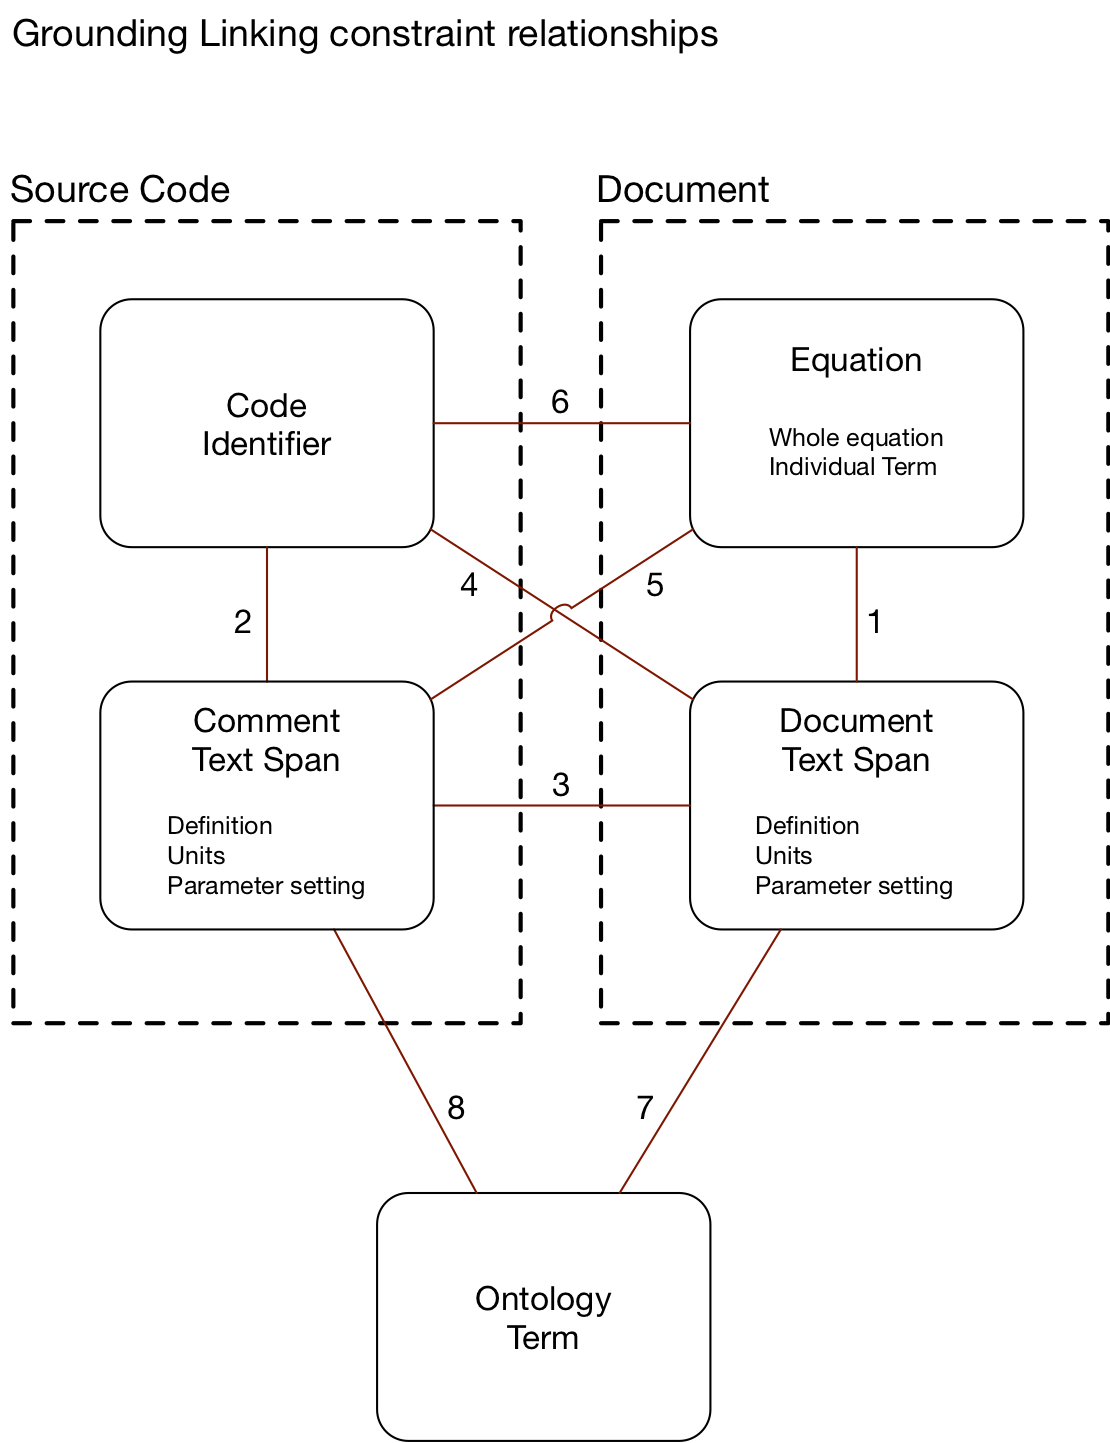
\includegraphics{figs/grounding.png}
\caption{Grounding concepts and elements by linking}
\end{figure}

There are four types of information source element types, coming from
two sources:

\begin{itemize}
\tightlist
\item
  Source code, which include

  \begin{itemize}
  \tightlist
  \item
    Code Identifiers
  \item
    Code Comments
  \end{itemize}
\item
  Documents, which include

  \begin{itemize}
  \tightlist
  \item
    Document text
  \item
    Equations
  \end{itemize}
\end{itemize}

Code comments and document text in turn express at least three kinds of
information:

\begin{itemize}
\tightlist
\item
  Descriptions (defintiions): associating a term with an expression,
  definition or definition of a concept.
\item
  Units: associating the scale or units of a quantity.
\item
  Parameter setting: expressing value constraints or specific values
  associated with a quantity.
\end{itemize}

Each link between source element types is made by a different inference
process that depends on the information available in the sources.

\begin{itemize}
\tightlist
\item
  Link type 1 involves associating equations and their component terms
  to concepts in text. The start of our approach to identifying these
  links is described in the next section.
\item
  Link type 2 involves associating code identifiers with concepts
  expressed in source code comments. In this phase, we infer these links
  by identifying mentions of the identifier names in source code text.
  In the future we will also make use of proximity of comments to
  locations in code as well as code scope to additionally support
  identifier-to-comment associations.
\item
  Link type 3 involves associating code comment and document text. This
  linking inference is performed using a similarity score based on text
  embedding distance.
\item
  Link types 4, 5 and 6 are mapped out here, but we do not yet provide
  inference methods for these.
\item
  Link types 7 and 8 involve mapping textual mentions of concepts to
  terms in one or more domain ontologies. We are working with Galois to
  demonstrate this in the September demo. The core approach will likely
  be an embedding similarity scoring, similar to the approach to Link
  type 3.
\end{itemize}

\hypertarget{text-and-equation-linking}{%
\subsection{Text and Equation Linking}\label{text-and-equation-linking}}

The team is working to not only extract variables from equations, but
also to link them to the in-text variables as well as the source code
variables. In order to evaluate the performance of the former, the team
has begun creating an evaluation dataset. The specific task the team is
looking to evaluate is linking the equation variables to their in-text
definitions (ex. 1) and, when present, the associated units (ex. 2).

\begin{figure}
\centering
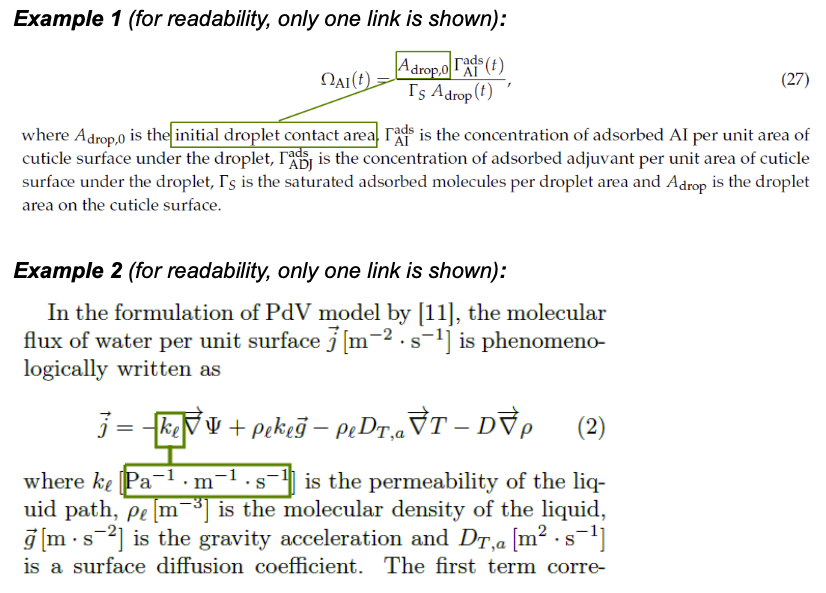
\includegraphics{figs/annotation_example.png}
\caption{Example of links}
\end{figure}

This effort will include the following steps: - (in progress) collecting
the documents to annotate: currently, the team is working on creating a
set of heuristics to select the documents most suitable for the
annotation exercise; - (in progress) creating the annotation guidelines:
the team is going through an iterative process of testing the guidelines
on a small number of annotators and adjusting the guidelines based on
the quality of elicited annotations, the level of agreement between the
annotators, and the annotators' feedback; - annotating the documents; -
calculating the inter-annotator agreement score as a measure of quality
of the created dataset.

Once completed, the team will use the collected dataset to evaluate
linking techniques.

\hypertarget{text-reading}{%
\section{Text Reading}\label{text-reading}}

The team has been working on improving the quality of the extraction of
variable units from text and comments.

\hypertarget{extracting-units-from-text}{%
\subsection{Extracting units from
text:}\label{extracting-units-from-text}}

\begin{figure}
\centering
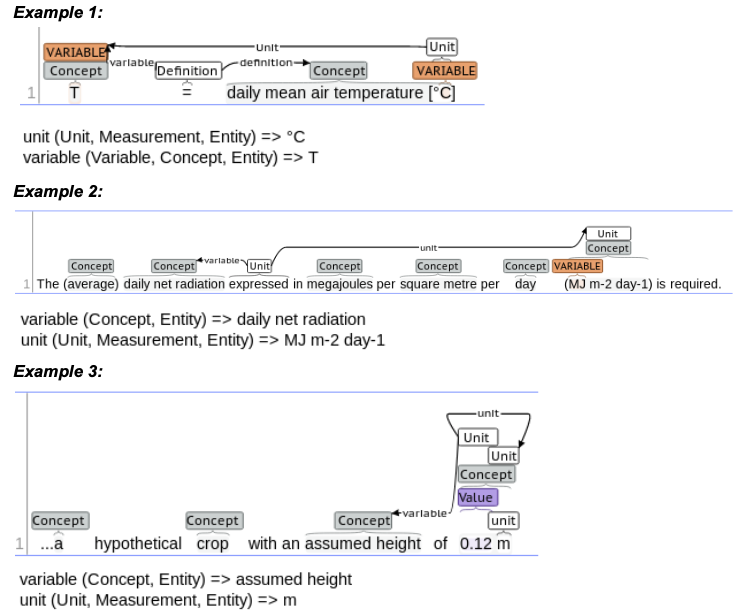
\includegraphics{figs/units_text.png}
\caption{Example units in text}
\end{figure}

Extracting units from scientific text (see examples above) is a
multi-step process. First, a number of basic units are extracted with a
lexicon-based entity finder; the lexicon has been recently updated to
exclude a number of basic units that resulted in false positives due to
their similarity to variables. Second, composite (i.e., multi-token)
units as well as units which are not in the lexicon, are extracted using
rules. False positives are eliminated by applying a set of heuristic
constraints (e.g., number of tokens in the candidate unit, length of
each token in the candidate unit, presence of digits, etc.). Finally,
units are attached to the relevant previously-found variables (ex. 1)
and concepts (exs. 2-3) with rules. Frequently, units occur in sentences
that do not include the relevant variable, with units attaching to the
variable definitions/concepts. To address this issue, the team will
start working on resolving these definitions/concepts to the relevant
variables in the surrounding text.

\begin{figure}
\centering
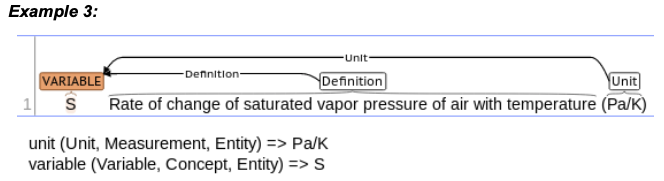
\includegraphics{figs/units_comment.png}
\caption{Example units in comments}
\end{figure}

With comments being less varied than text, extracting units from
comments happens in only two stages: extracting units with a rule and
attaching the unit to the previously found variable with another rule
(see example above).

\hypertarget{equation-reading}{%
\section{Equation Reading}\label{equation-reading}}

Now that the team has a fully working implementation of the im2markup
model, they have formatted and normalized data from one year of arxiv to
use for training. This amounts to over 1.1M equation examples, an order
of magnitude more training data than was used in the original and the
newly gathered data represents a wide variety of domains (as compared to
the original data which was only from particle physics). The team is
currently training a model on this larger dataset.

Additionally, the team is working on data augmentation, as previously
mentioned, and to complement that effort, they are beginning to
implement the Spatial Transformer Network (STN; Jaderberg et al., 2015).
The STN is a differentiable module which learns to predict a spatial
transformation for each image independently, in order to make the model
as a whole invariant to any affine image tranformation, including
translation, scaling, rotation, and shearing. One advantage of the STN
is that it is trained end-to-end with the rest of the model, not
requiring direct supervision. Instead it will learn to transform the
image in such a way that the end task performance improves.

Jaderberg, M., Simonyan, K., \& Zisserman, A. (2015). Spatial
transformer networks. In Advances in neural information processing
systems (pp.~2017-2025).

\hypertarget{model-analysis}{%
\section{Model Analysis}\label{model-analysis}}

\hypertarget{domain-constraint-propagation}{%
\subsection{Domain Constraint
Propagation}\label{domain-constraint-propagation}}

\hypertarget{task-overview}{%
\subsubsection{Task Overview}\label{task-overview}}

The overall goal of the domain constraint propagation task is to find
the minimum functional bounds on each of the inputs for a GrFN such that
no set of input values will fail to evaluate due to a mathematical
error. Concretely, minimal functional bounds are bounds that arise upon
the inputs to a given computation because of the functions computed in
the course of that computation. An example of this would be the
\texttt{arcsine} function, whose domain is \texttt{{[}-1,\ 1{]}}. If the
following function were present in source code,
\texttt{y\ =\ arcsine(x)} then a constraint would be placed on the
domain of \texttt{x} such that it would be \texttt{{[}-1,\ 1{]}} at
most. In general, programs extracted from the Program Analysis team are
likely to have complex interactions between variables and mathematical
operations that lead to domain constraints. This means that the domain
constraints of a single variable are likely going to be in terms of the
other variables. This means that solutions to our domain constraint
propagation problem will likely be in the form of a constraint
satisfaction problem (CSP) with variables that have infinite domains.
Normally time complexity is a concern for CSP problems even upon finite
domains; however, those time constraints are associated with determining
if the set of constraints has a solution. Our intended use case for this
is as a recognizer for whether a set of input values will cause a
mathematical error in calculation, so we need not worry about the widely
studied time complexity concerns associated with CSPs.

The following are all true about domain constraints derived from the
computations found in source code: 1. Some mathematical functions
\emph{set} domain constraints upon the variables in their child
structures. 2. Some mathematical functions \emph{translate} domain
constraints upon the variables in their child structures. 3. Some
mathematical functions create complex multi-interval domain constraints.
4. Conditional evaluations introduce multiple possible domain
constraints over for a variable

From fact \texttt{1} items we see that the domain constraint for a
particular variable will be set by mathematical functions that impose
constraints on their inputs, such as arccosine and the logarithm
function. These constraints will be in the form of mathematical domain
intervals. Other operators will shift or scale the domain constraints
intervals upon a variable, such as the addition, multiplication, and
exponentiation operators. Fact \texttt{3} shows us that a particular
variables domain could be a series of intervals. This can occur due to
functions that impose domains with holes, such as the division
operation. Now a domain constraint upon a variable can be described as a
list of domain intervals for an input variable over which the output can
be computed. But, as mentioned by fact \texttt{4}, the presence of
conditionals adds complications to the domain constraints for a
variable. Now the domain constraint must be based on the conditional
evaluation in cases where two separate mathematical functions make use
of a variable in a constrained manner as governed by a conditional.
Since our plan is to use the domain constraints discovered during the
propagation process to validate input sets, we will use the most
restrictive case for conditionals which will be to require any variable
domains found under conditionals to fulfill the constraints of all
branches of the conditional.

\hypertarget{algorithmic-solver-approach}{%
\subsubsection{Algorithmic Solver
Approach}\label{algorithmic-solver-approach}}

Our approach to solving the domain constraint propagation problem will
be to create an algorithmic solver that uses the structure of the source
code that we extract our models from in order to create a graph of the
constraints upon the domains of different variables. The algorithmic
solver will perform a line-by-line walk through the code, and will
perform a tree-walk at each line of the code, generating and updating
variable constraints upon visiting operators on each line. To visualized
the tree-walk that will occur for each line of code, consider the
example complex mathematical equation shown below.

\begin{Shaded}
\begin{Highlighting}[]
\NormalTok{a }\OperatorTok{=}\NormalTok{ arccosine(logarithm((x}\OperatorTok{*}\NormalTok{y)}\OperatorTok{/}\DecValTok{5}\NormalTok{)) }\OperatorTok{*}\NormalTok{ square_root(z)}
\end{Highlighting}
\end{Shaded}

This can be rewritten in the following form with only one mathematical
operation per-line to show how a tree-walk will occur:

\begin{Shaded}
\begin{Highlighting}[]
\NormalTok{(}\DecValTok{1}\NormalTok{) n0 }\OperatorTok{=}\NormalTok{ x }\OperatorTok{*}\NormalTok{ y}
\NormalTok{(}\DecValTok{2}\NormalTok{) n1 }\OperatorTok{=}\NormalTok{ n0 }\OperatorTok{/} \DecValTok{5}
\NormalTok{(}\DecValTok{3}\NormalTok{) n2 }\OperatorTok{=}\NormalTok{ logarithm(n1)}
\NormalTok{(}\DecValTok{4}\NormalTok{) n3 }\OperatorTok{=}\NormalTok{ arccosine(n2)}
\NormalTok{(}\DecValTok{5}\NormalTok{) n4 }\OperatorTok{=}\NormalTok{ square_root(z)}
\NormalTok{(}\DecValTok{6}\NormalTok{) a }\OperatorTok{=}\NormalTok{ n3 }\OperatorTok{*}\NormalTok{ n4}
\end{Highlighting}
\end{Shaded}

If we evaluate, in a similar manner as the tree-walk will occur, from
line 6 backwards to line 1 we can see how the domain constraints will
propagate to the input variables, such as how the domain constraint
introduced by \texttt{arccosine} is propagated from
\texttt{n2\ -\/-\textgreater{}\ n1\ -\/-\textgreater{}\ n0\ -\/-\textgreater{}\ x\ \&\ y}.
Just as this process has been carried out for a single line mathematical
function, the same tree-walk can be done across lines to propagate
variable constraints backwards to all the input variables of a
scientific model. Using this method works very well for straight-line
code; however there are atleast two questions that still need to be
answered: 1. How will this method work for function calls? 2. How does
this method handle loops?

For problem \texttt{1}, if we can observe the code for a function call
then we can treat the function exactly the same as we would
straight-line code. If we cannot observe the code for a function call,
but we do know it's domain/range then we can treat this function just
like any other mathematical operator upon its inputs and outputs.
However, if we cannot observe the functions code and we do not have any
information of its inputs or outputs then we will be unable to determine
the validity of solutions to the domain constraint problem. For problem
\texttt{2}, if we know the number of times we are expected to loop then
we can guarantee whether input sets satisfy the domain constraints;
otherwise, we can perform this analysis on the loop as though it is
straight-line code with a conditional.

\end{document}
